\section{Globales FEM}
Wie in der Aufgabenstellung beschrieben, soll zur Überprüfung der Handrechnungen und zur Bestimmung von Schnittgrössen ein globales FEM-Modell zur Anwendung kommen. In diesem Kapitel wird nun beschrieben, wie dieses FEM-Modell aufgesetzt und welche vereinfachenden Annahmen getroffen werden. Weiter werden die Ergebnisse der Simulationen aufgeführt und mit den Handrechnungen verglichen und beurteilt.

Analog zu den Handrechnungen werden vier verschiedene FEM-Berechnungen durchgeführt, welche jeweils ein Lastfall der Beschleunigung des Modus \emph{A} genauer untersuchen.\\

Mit dem globalen FEM-Modell sollen folgende Punkte bestimmt werden:
\begin{itemize}
  \item Lagerreaktionen
  \item Maximale Axialkräfte, Querkräfte und Biegemomente in Chassis, Dach und den Trägern A und B
  \item Kontaktreaktion: Verbindung Chassis zu Träger A und B
  \item Kontaktreaktion: Verbindung Chassis zu Boden
  \item Deformation
\end{itemize}

\subsection{Idealisierung und Modell}
Der Solar Butterfly wird, wie in den Handrechnungen, als \glqq Kasten\grqq{} betrachtet und mit Balken und Schalen idealisiert. Das Chassis, die Deichsel, die Träger A und B sowie die Dachträger werden als Balkenelemente (Beam) mit den entsprechenden Querschnitten modelliert. Die Wände, Dächer und der Boden werden als Schalenkörper (Shell) modelliert, wobei den Schalenkörper jeweils ein Lagenaufbau (Layered Section) zugewiesen wird, welcher ihre Sandwichbauweise nachahmt. In der Abbildung \ref{FEM Mesh1} ist das komplette Modell des Solar Butterflys dargestellt. In der Abbildung \ref{FEM Mesh3} wurden die Schalenkörper ausgeblendet, sodass nur die Balkenelemente sichtbar sind.

\begin{figure}[H]
  \centering
  \centering
  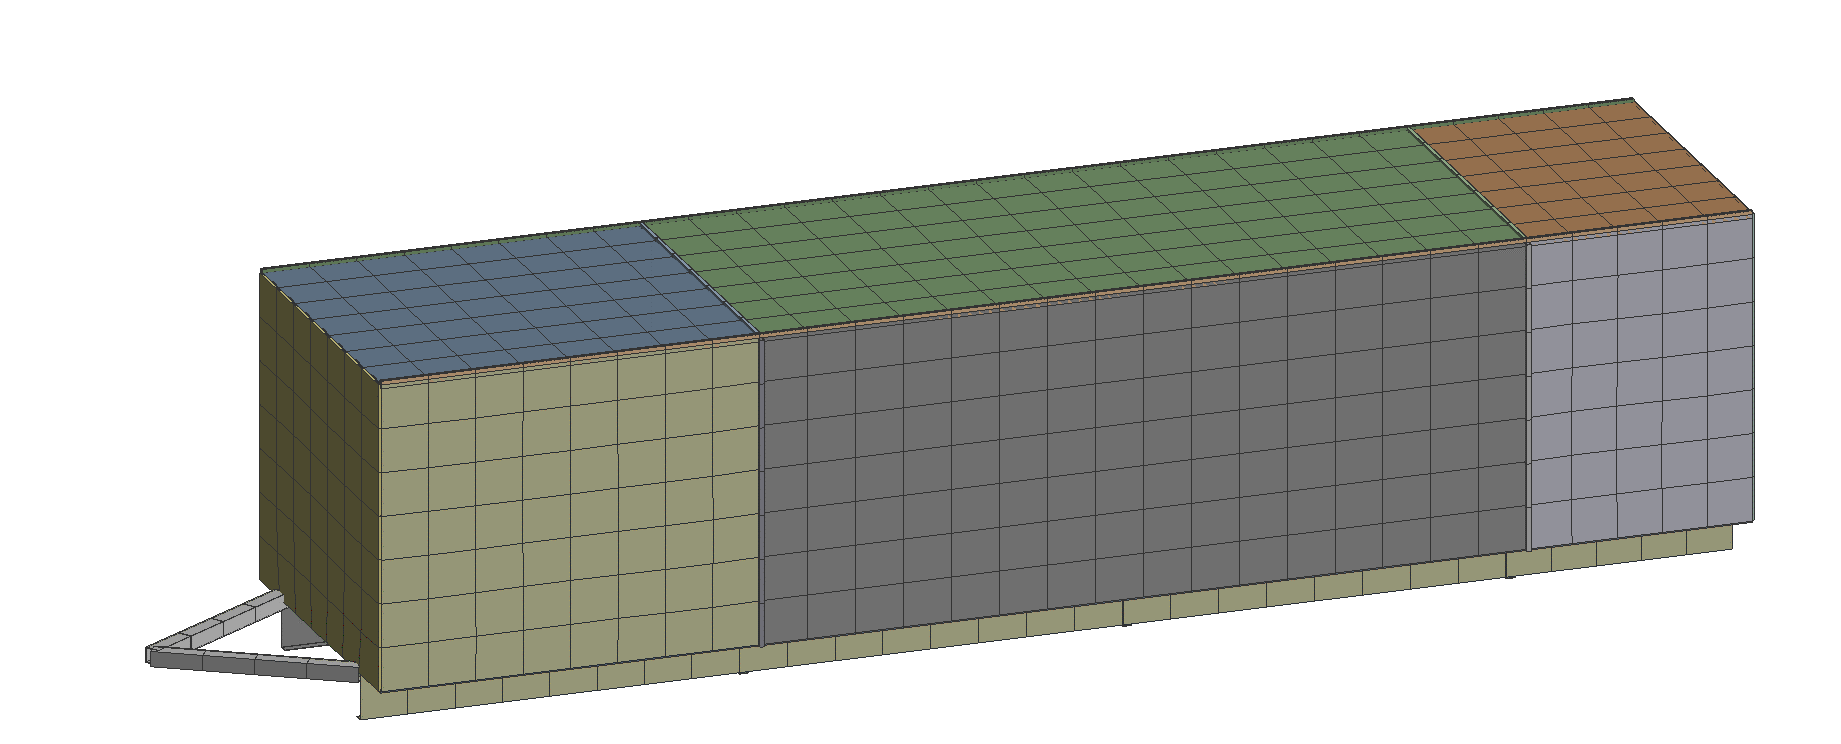
\includegraphics[width=.8\linewidth]{04_figures/FEM Mesh1.png}
  \caption{Darstellung der Balken und Schalenkörper im FEM-Modell}
  \label{FEM Mesh1}
\end{figure}
\begin{figure}[H]
  \centering
  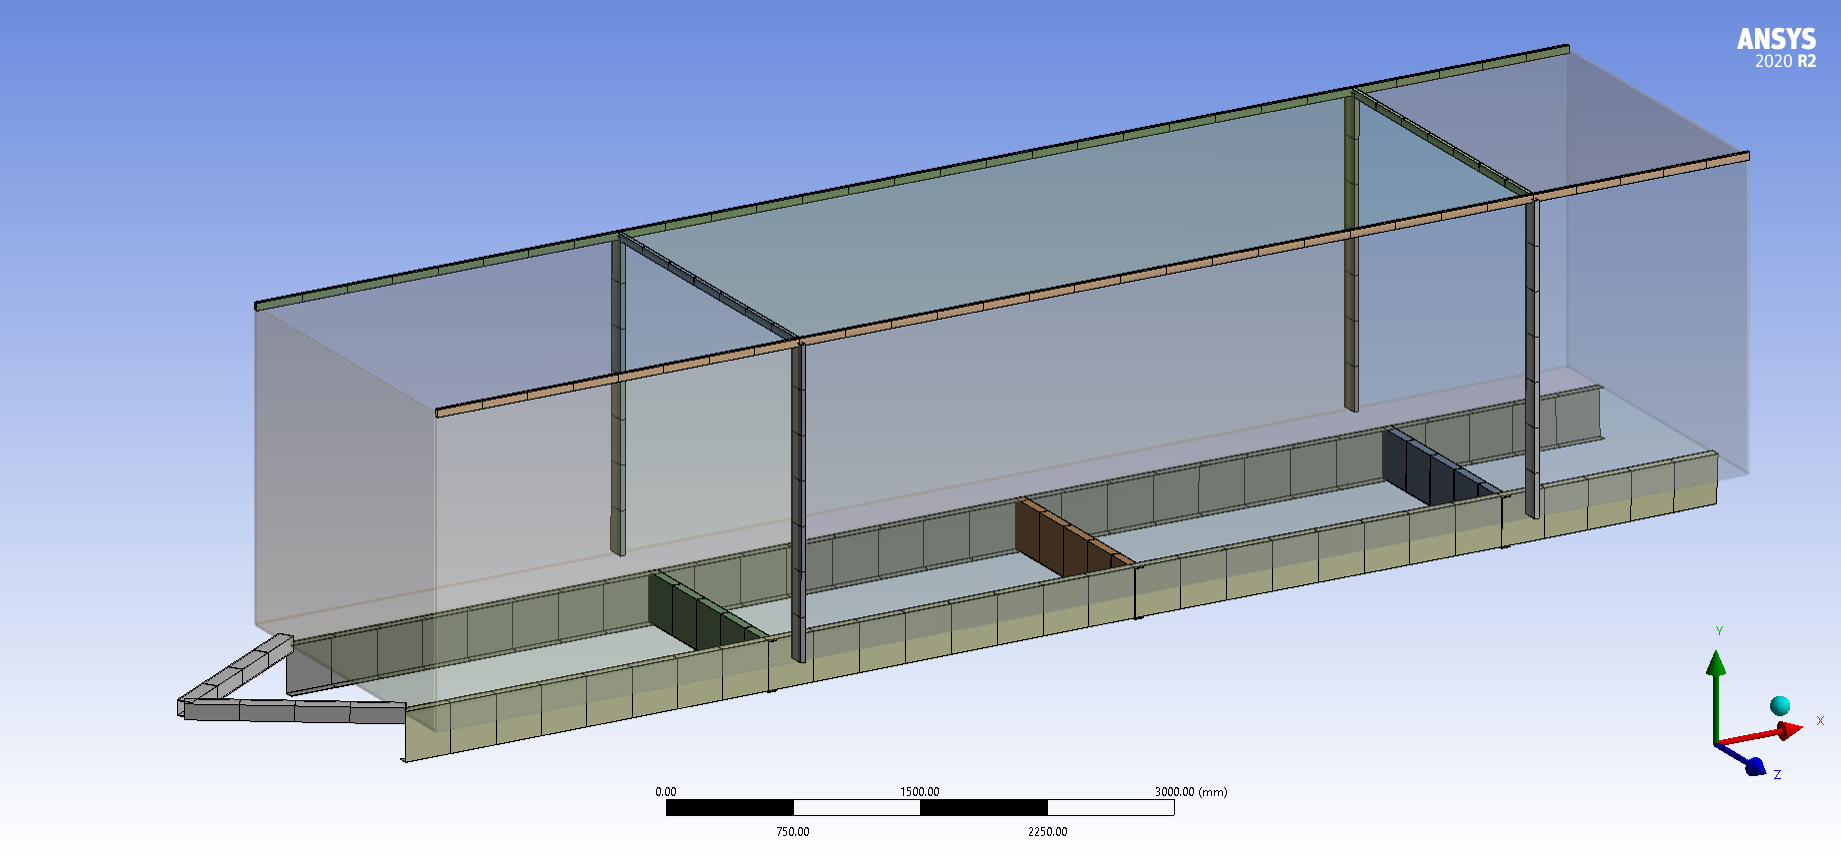
\includegraphics[width=.8\linewidth]{04_figures/FEM Mesh3.png}
  \caption{Darstellung der als Balken idealisierten Körper}
  \label{FEM Mesh3}
\end{figure}

Um die Masse des Solar Butterflys modellieren zu können, werden, zusätzlich zu den Massen der modellierten Bauteile, Punktmassen (Point Mass) eingeführt. Es werden für die drei Raumelemente Küche, Mittelkörper und Bad je eine Punktmasse definiert, deren Masse und Trägheitsmomente mit der Hilfe der Massenverteilung aus dem Kapitel \ref{Massenverteilung} bestimmt werden. In der Abbildung \ref{img:FEM Punktmasse} sind die Verbindungen der Punktmassen mit dem Rest des Modelles dargestellt. Sie werden über das Chassis, die Träger A und B, sowie über die Verbindungsstellen wischen den Wänden und dem Boden getragen.\\
\begin{figure}[H]
  \centering
  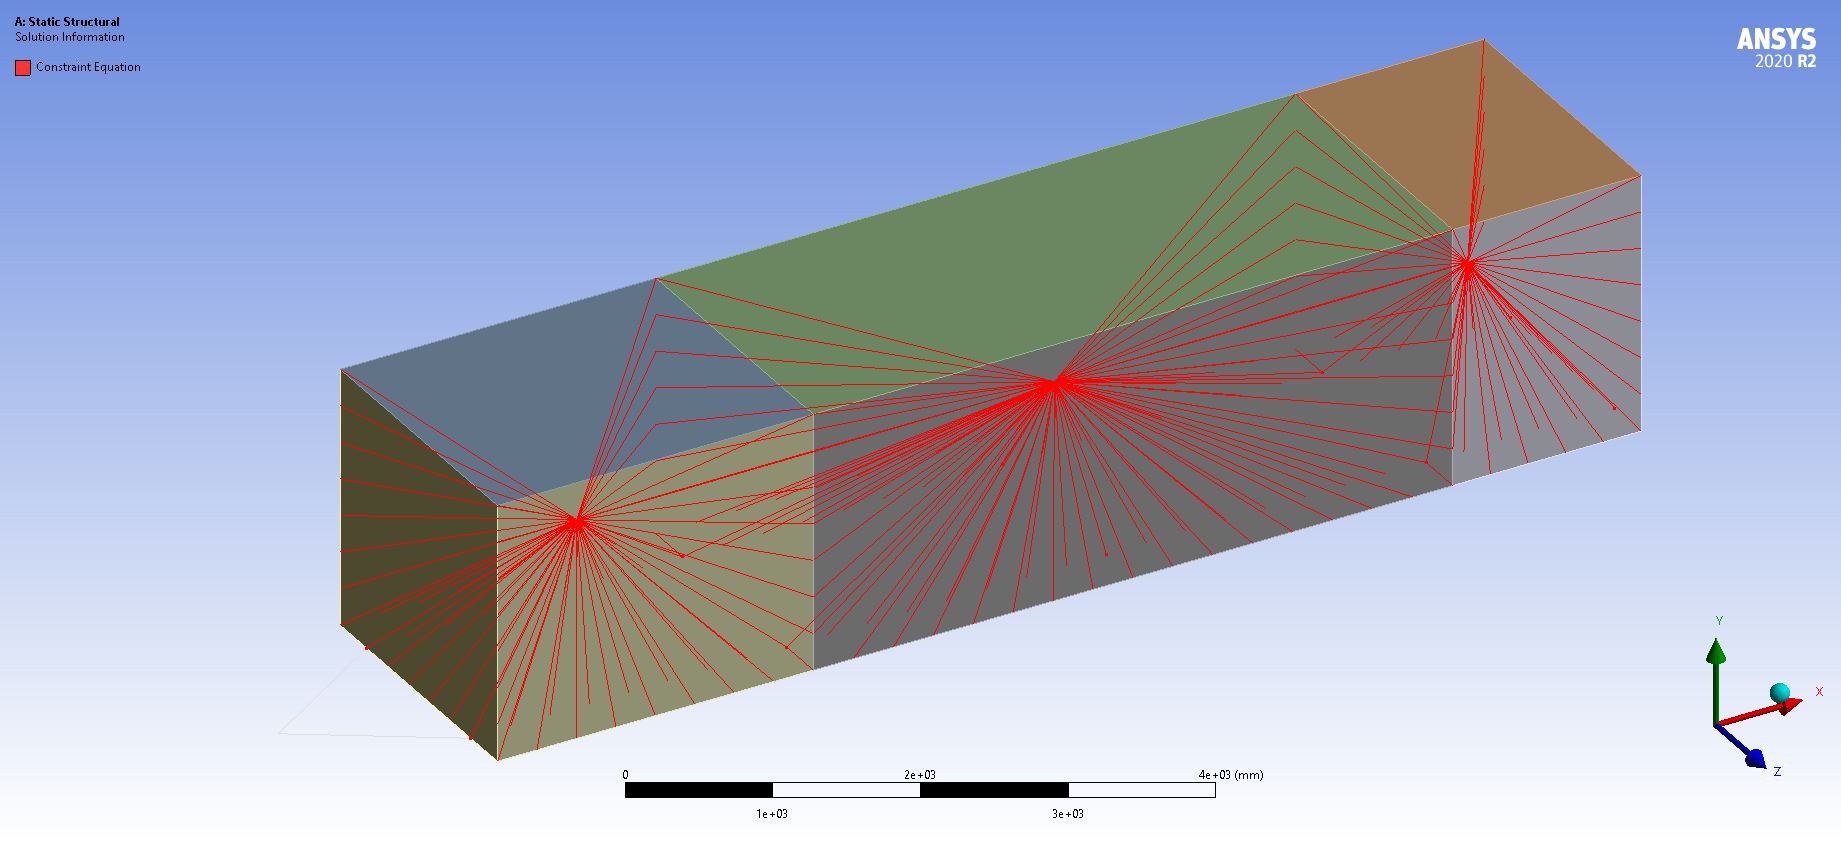
\includegraphics[width=0.8\linewidth]{04_Figures/FEM Punktmasse.png}
  \caption{Verbindungen der Punktmassen zum Rest des Modelles}
  \label{img:FEM Punktmasse}
\end{figure}

Die Deichsel, Längsträger und Querträger des Chassis werden durch das Zusammenführen der deckungsgleichen Koten miteinander verbunden (Node Merge). Auf die selbe Art und Weise werden die Träger A und B, die Träger des Daches sowie der Boden, die Wände und das Dach des Aufbaus miteinander verbunden. Der verbundene Aufbau wiederum wird auf zwei Arten mit dem Chassis verbunden. Einerseits werden die Träger A und B über einen \emph{Fix-Joint} (Body-Body Verbindung, alle Freiheitsgrade eingeschränkt) an ihrem untersten Knoten mit dem Chassis verbunden. Weiter wird der Boden über \emph{General-Joint}-Verbindungen%Fussnote...
\footnote{Die \emph{General-Joint}-Verbindungen wurden mit der Hilfe von \emph{Named Selections} und der \emph{Object Generator} Funktion erstellt. Die Kraftreaktionen wurden durch die Parametrisierung der Ergebnisse ausgelesen.}
(Body-Body Verbindung, die rotatorischen Freiheitsgrade sind frei, die translatorischen eingeschränkt.) mit den Längsträgern des Chassis verbunden. Insgesamt ist der Boden an jedem Längsträger über 30 Knotenverbindungen it dem Chassis verbunden. Sie repräsentieren die Klebestellen zwischen Boden und Chassis.\\
In allen folgenden beschriebenen FEM-Simulationen ist der Solar Butterfly analog zu den Handrechnungen im Kapitel \ref{sub:Longitudinale Beschleunigung} (Lastfall \emph{1.1 Vertikale Beschleunigung}) gelagert. Am Spitz der Deichsel sind die rotatorischen Freiheitsgrade frei, die translatorischen jedoch eingeschränkt. An der Achse wird lediglich die Verschiebung in x-Richtung (Fahrtrichtung) zugelassen.


\subsection{Ergebnisse}
Im Anhang \ref{FEM Ergebnisse} sind die Ergebnisse der FEM-Berechnungen Tabellarisch festgehalten. Sofern für die ausgelesenen Grössen Handrechnungen durchgeführt wurden, sind deren Ergebnisse ebenfalls in den besagten Tabellen zu finden, sodass diese direkt mit den Ergebnissen der FEM-Berechnungen verglichen werden können. Die Schnittkräfte und Kontaktreaktionen der Tabellen beziehen sich jeweils auf einen einzelnen Balken oder Verbindung. Die Kontaktreaktion zwischen Chassis und Boden bezieht sich auf eine einzelne Knotenverbindung. Die in den Tabellen aufgeführten Werte stellen jeweils den Maximalwert dar.\\
Im Anhang \ref{FEM Deformation} sind Bilder, welche die Deformation des Solar Butterflys dokumentieren, zu finden. Die FEM-Datei ist im elektronischen Anhang \ref{e:Globales FEM} angefügt. Die Auswertung der Ergebnisse wurde mit einer Exceltabelle durchgeführt, welche im elektronischen Anhang \ref{e:FEM Auswertung} zu finden ist.

\subsubsection{Vergleich mit Handrechnungen}
Im Lastfall \emph{1.1 Vertikale Beschleunigung} sind die berechneten Axialkräfte (15.8 kN) im Dach rund acht Mal so hoch, wie jene des FEM-Modelles (1.9 kN). Dies ist vermutlich darauf zurückzuführen, dass das mittragende Dach, welches ebenfalls Axialkräfte aufnimmt, in den Handrechnungen nicht mitberücksichtigt wurde.\\
Im Lastfall \emph{1.4 Laterale Beschleunigung} sind die mit der FEM-Berechnung erhaltenen Axialkräfte im Chassis und den Längsträger des Daches gut drei Mal höher als jene der Handrechnungen. Dies, da sich der Solar Butterfly unter lateraler Beschleunigung, nicht wie angenommen verbiegt, sondern verdreht. Die Art der Deformation ist ähnlich wie jene im Lastfall \emph{1.5 Rotatorische Beschleunigung} (vgl. Abbildungen \ref{FEM 1.4} und \ref{FEM 1.5} im Anhang \ref{FEM Deformation}). Da diese grundlegende Annahme der Auswirkungen der Belastung falsch getroffen wurde, sind die Ergebnisse auch dem entsprechend unterschiedlich. Die erhaltenen Kräfte sind in ihrer Art vergleichbar mit jenen des Lastfalles \emph{1.5 Rotatorische Beschleunigung}, im Betrag liegen sie jedoch tiefer.\\

\subsubsection{Beurteilung Dach}
In der folgenden Tabelle sind die Schnittgrössen der Träger des Daches enthalten.

\begin{table}[H]
\centering
\begin{tabular}{lccccccc}
\thickhline
  &	Einheit	&	1.1	&	1.3	&	1.4	&	1.5	&	Max	&	Min	\\	\hline
Axialkraft	&	N	&	1949	&	1551	&	-1731	&	-2450	&	1949	&	-2450	\\
Querkraft	&	N	&	108	&	55	&	14	&	32	&	108	&	14	\\
Biegemoment	&	kNmm	&	17	&	17	&	9	&	19	&	19	&	9	\\	\thickhline
\end{tabular}
\caption{Schnittgrössen des Daches in den unterschiedlichen Lastfällen}
\label{tab:FEMres Dach}
\end{table}


Wie im Kapitel \ref{sec:Dach} beschrieben, ist das dimensionierende Kriterium des Daches dessen Verformung aufgrund des Eigengewichtes. Dem entsprechend stellen die in der Tabelle \ref{tab:FEMres Dach} aufgeführten Schnittgrössen keine kritischen Lasten dar und werden hier nicht vertieft aufgegriffen. Die FEM-Ergebnisse zeigen, dass verfolgte Konzept die Dachträger nicht optimal ausnützen.

Das Potential der Gewichtsoptimierung des Daches wird als gering eingestuft. Auch wenn die Träger des Daches global gesehen überdimensioniert sind, werden über sie, im eingefahrenen Zustand, die seitlichen Raumelemente befestigt und gesichert. Sie übernehmen somit eine zusätzliche Funktion. Würde ein anderes Konzept zur Versperrung der seitlichen Raumelementen ausgearbeitet, könnte das Dach eventuell auf eine andere Weise optimaler versteift (z.B. mit aufgeklebten CFK-Hutprofilen) und die Dachträger weggelassen werden. Die Funktionen (Versteifung und Versperrung) könnten so getrennt und jeweils optimaler erfüllt werden.\\
Wird vom jetzigen Konzept noch weiter abgewichen und der Entwurf des unterbrochenen Daches (4 GFK-Sandwichpanelen à ca. 2 x 1.3 m im mittleren Raumelement) verworfen, gäbe es allenfalls die Möglichkeit, ein durchgehendes Dach in Sandwichbauweise zu verwenden. Dieses könnte, ähnlich wie der Boden, mit Ocean-PET und Aluminium-Deckschichten in einem Stück gefertigt und mit Hartschaum-Einsätzen und Verstärkungen individuell angepasst und optimiert werden.
Bei der Fertigung solcher Sandwichstrukturen können direkt Gehrungen gefräst werden, welche als Plattenabschluss und allenfalls auch als Halterung für Verschliessmechanismen benützt werden können.\\
Der Nachteil dieses Konzepts ist jedoch, dass nicht die Standard-Solarmodule verwendet werden können, welche von Beginn an des Projektes als vorgegeben betrachtet wurden (Sponsoring). Es stellt sich entsprechend die Frage, zum Einen \emph{wer} und \emph{wie} die Solarzellen auf das Dach laminiert werden, da diese nicht direkt im Herstellungsprozess der Sandwichkonstruktion mitlaminiert werden können. Dass die Solarzellen unter Umständen \glqq von Hand\grqq{} auf das Dach laminiert werden müssen, könnte sich aufgrund der Flexibilität bezüglich Dimensionierung und Verkabelung, auch als Vorteil erweisen. Als weiterer Vorteil ist zu ergänzen, dass die Verbindungsstellen zwischen den Solarpanelen und Träger, sowie zwischen den einzelnen Solarpanelen, wegfallen würden.\\
Auch wenn die Gewichtsersparnisse vermutlich gering sind (oder wohl möglich auch nicht vorhanden sind), würde die Komplexität reduziert werden können. Die Verbindungsstellen würden wegfallen und die Anzahl der Bauteile würde reduziert werden.


\subsubsection{Beurteilung Träger A und B}
In der Tabelle \ref{tab:FEMres Träger} sind die maximalen Schnittgrössen der Träger A und B zusammengestellt.
\begin{table}[H]
\centering
\begin{tabular}{lccccccc}
\thickhline
	&	Einheit	&	1.1	&	1.3	&	1.4	&	1.5	&	Max	&	Min	\\	\hline
Axialkraft	&	N	&	-10846	&	1551	&	2654	&	-4066	&	2654	&	-10846	\\
Querkraft	&	N	&	93	&	55	&	1071	&	1311	&	1311	&	55	\\
Biegemoment	&	kNmm	&	326	&	17	&	639	&	788	&	788	&	17	\\	\thickhline
\end{tabular}
\caption{Schnittgrössen der Träger in den unterschiedlichen Lastfällen}
\label{tab:FEMres Träger}
\end{table}


Die maximale Axialkraft von -10.8 kN hat, bei einer Querschnittsfläche eines Trägers von rund 1180 $mm^2$, Druckspannungen von 9.2 MPa zur Folge. Die Gefahr des Knickens ist nicht vorhanden, da die Träger auf mindestens zwei Seiten über die Wände gestützt werden und die Druckbelastung im Verhältnis zum Flächenträgheitsmoment des Trägers eher tief ist (Knickung nach Euler). Das Maximale Biegemoment von 772 kNmm führt, bei einem minimalen Widerstandsmoment von 11900 $mm^3$, zu Spannungen in der Höhe von 65 MPa.\\
Ob die Dimensionen der Träger A und B optimal gewählt wurden lässt sich anhand der FEM-Ergebnissen nicht beurteilen, da angenommen wird, dass die dimensionierenden Belastungen währen dem Ausfahren der seitlichen Raumelementen (Modus B3) auftreten. Es wird daher empfohlen in einem weiteren Schritt ein globales FEM-Modell für den Modus B3 zu erstellen und dieses zu analysieren. Es kann jedoch gesagt werden, dass die überprüften Lastfälle keine kritischen Belastungen für die Träger A und B darstellen, diese jedoch auch nicht grob überdimensioniert sind. Dem entsprechend kann das Potential zur Gewichtseinsparung nur schwer abgeschätzt werden.

\subsubsection{Verbindung Boden zu Chassis}
In der folgenden Tabelle sind die maximalen Kontaktreaktion und Spannungen der Verbindung zwischen Chassis und Boden zu finden.

\begin{table}[H]
\centering
\begin{tabular}{lcccccc}
\thickhline
	&	Einheit	&	1.1	&	1.3	&	1.4	&	1.5	&	Max	\\	\hline
Normalkraft (Zug)	&	N	&	883	&	288	&	1942	&	3118	&	3118	\\
Schubkraft (xz-Ebene)	&	N	&	9933	&	1731	&	10972	&	10761	&	10972	\\	\hline
Normalspannungen	&	MPa	&	0.05	&	0.02	&	0.11	&	0.17	&	0.17	\\
Schubspannungen	&	MPa	&	0.56	&	0.10	&	0.61	&	0.60	&	0.61	\\	\thickhline
\end{tabular}
\caption{Kontaktreaktion und Spannungen der Verbindung zwischen Chassis und Boden in den unterschiedlichen Lastfällen}
\label{tab:FEMres Boden}
\end{table}


Wird die Klebefläche des Chassis auf die 60 Knotenverbindungen verteilt ergibt sich eine Fläche von 17880 $mm^2$ pro Knotenverbindung. Mit den in der Tabelle \ref{tab:FEMres Boden} angegebenen Kontaktreaktionen ergeben sich somit maximale Normalspannungen von 0.17 MPa und maximale Schubspannungen von 0.61 MPa. Die Normalspannungen liegen unterhalb den Design-Allowables und die Schubspannungen jedoch deutlich darüber. Hierbei muss zusätzlich angemerkt werden, dass aufgrund der mangelnden Auflösung (30 Knoten pro Längsträger des Chassis verteilt auf ca. 9 m) und nicht optimaler Modellierung, lokal die Spannungen deutlich höher liegen könnten und dass das verwendete Modell nicht geeignet ist, um diese Spannungskonzentrationen festzustellen.\\
Würde die FEM-Berechnung erneut durchgeführt werden, wird empfohlen, das Chassis mittels Schalenkörper zu modellieren, wodurch eine Kontakt-Verbindung (an Stelle einer Joint-Verbindung) verwendet werden könnte. Eine weitere Möglichkeit wäre, die Klebeverbindung mittels MPC-Kontakte (MPC184 Elementen) mit definierbarer Steifigkeit zu modellieren, was als eine exaktere Modellierung erachtet wird.

Um die Klebeverbindung und die darin erlangten Spannungen besser beurteilen zu können, müssten unterschiedliche Klebstoffe in Betracht gezogen und deren Design-Allowables bestimmt werden. Es wurde sich nicht vertieft mit Klebstoffen auseinandergesetzt, sodass die Klebstoff-Design-Allowables keine abschliessende Werte darstellen. Dennoch werden sie als gute Näherung erachtet sodass erwartet wird, dass die Festigkeitswerte anderer Klebstoffe in der Selbe Grössenordnung liegen.\\
Auch wenn bessere Klebstoffe gefunden werden könnten, ist die Klebeverbindung, aufgrund der vielen unbekannten Grössen und mangelnder Erfahrung, als Risiko zu betrachten und muss in einem weiteren Schritt genauer untersucht werden. Für das weitere Vorgehen wird, je nach zur Verfügung stehender Zeit, empfohlen auf eine alternative Verbindungsmethode wie Nieten oder Schrauben zu wechseln oder Personen und Firmen mit den benötigten Erfahrungen auf diesem Gebiet dem Projekt zur Unterstützung beizuziehen.\\
Es müssen auf jeden Fall weitere Untersuchungen und Abklärungen vorgenommen werden, bevor ein definitiver Entscheid getroffen oder mit der Herstellung des Solar Butterflys begonnen wird.

\subsubsection{Verbindung Träger A und B zu Chassis}
In der Tabelle \ref{tab:FEMres Träger Kont} im Anhang \ref{sec:FEMres Träger} sind die maximalen Kontaktreaktionen der Fixed-Joint-Verbindungen zwischen den Trägern A und B und dem Chassis zu finden.\\
Die Idealisierung der Verbindungen stellt eine schlechte Abbildung der wirklichen Verbindung dar. So sind die Träger A und B zum Beispiel in der Realität direkt am Chassis befestigt nicht wie modelliert, mit einem Abstand von ca. 400 mm (vlg. Abbildung \ref{FEM Mesh3}). Dieser zusätzliche Hebelarm verfälscht Biegemomentreaktionen sehr, sodass zu ihnen keine Aussagen gemacht werden.\\
Bei den Axialkräften der Verbindung wird angenommen, dass diese nicht stark verfälscht werden und dass sie für eine grobe Auslegung der Verbindung benütz werden können. Die maximale Axialkraft tritt mit 15.8 kN in negativer y-Richtung (Nach unten) im Lastfall \emph{1.1 Vertikale Beschleunigung} auf.


\subsubsection{Deformationen}
\label{Deformation}
Die FEM-Berechnungen zeigen, dass das Chassis, im Bezug auf das Übernehmen von Lasten, eine wichtigere Funktion übernimmt als zuvor angenommen. Die tragende Funktion des Aufbaus wurde wiederrum überschätzt. Diese Feststellung lässt sich unteranderem an der Abbildungen \ref{Def3} anhand der Deformationen erkennen. Das Chassis verformt sich relativ stark, während der Aufbau seine rechteckige Form nahezu beibehält. Besonders in den Lastfällen der lateralen und rotatorischen Beschleunigung ist zu erkennen, dass sich lediglich das Chassis stark verdreht, und nicht wie angenommen der komplette Solar Butterfly. Dies zeigt, dass die Eigenschaft des Chassis bezüglich Steifigkeit, im Vergleich zum Aufbau, eine entscheidende Rolle spielt. \\

\begin{figure}[H]
  \centering
  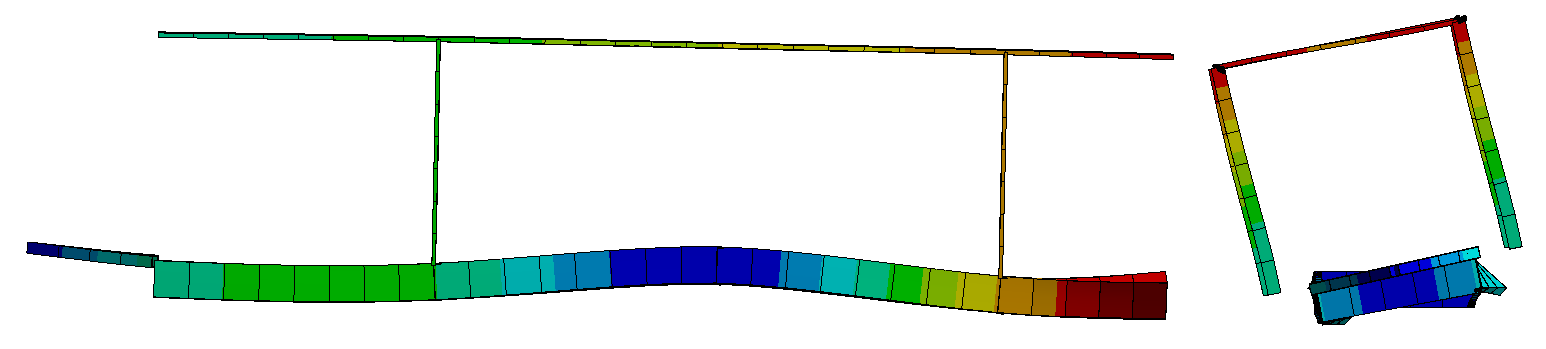
\includegraphics[width=.98\linewidth]{04_figures/Def3.png}
  \caption{Deformation des Solar Butterflys in den Belastungsfällen 1.1 Vertikale Beschleunigung (links) und 1.5 Rotatorische Beschleunigung (rechts). In den Darstellungen wurden die Schalenelemente ausgeblendet.}
  \label{Def3}
\end{figure}

Es ist jedoch nicht klar, ob dieses Ergebnis zum Teil auch auf die Art der Einbindung der Punktmassen ins FEM-Modell zurückzuführen ist. Oder anders ausgedrückt: es ist nicht klar, ob das selbe Ergebnis erzielt werden könnte, wenn die Massen realitätsgetreuer modelliert und ins Modell eingebunden worden wären. So befindet sich in der Realität ein grösserer Teil der Masse, in Form der ausfahrbaren Solarmodulen und den dazugehörigen Antriebselementen, an den Wänden des Solar Butterflys und nicht, wie modelliert, in den Zentren der Raumelemente.
Die Masse der ausfahrbaren Solarmodulen muss über die Wände und Träger A und B, zu einem gewissen Ausmass auch über das Dach, getragen und dessen Trägheitskräfte auf das Chassis übertragen werden. Die Punktmassen sind jedoch fast ausschliesslich direkt über das Chassis und die Träger A und B befestigt worden. Durch eine exaktere Verteilung und Einbindung der Massen ins Modell, würde sich der Lastpfad entsprechend verändern, was andere FEM-Ergebnisse hervorbringen würde.
Es ist wahrscheinlich, dass der Aufbau in der Realität eine tragendere Funktion übernimmt, als dies durch die FEM-Berechnungen gezeigt wird und dass dessen Deformation stärker ausfallen würde.\\
Auch wenn mit einer exakteren Modellierung gezeigt werden könnte, dass der Aufbau eine wichtigere Rolle übernimmt als dies durch die vorliegenden FEM-Berechnungen nahegelegt wird, steht fest, dass die Eigenschaften des Chassis das Verhalten des Solar Butterflys dominieren.\\

Das Gewicht des Chassis beansprucht mit 650 kg rund ein Viertel des Gewichtlimits für Europa von 2200 kg. Weiter handelt es sich beim Chassis um ein \glqq Standard-Chassis\grqq{}, welches nicht spezifisch für die Anwendung in diesem Projekt ausgelegt und optimiert wurde. Ferner wird der Boden zur Zeit nicht optimal ausgenützt. So entspringt die dimensionierende Grösse des Bodens aus einem Missbrauchslastfall (\glqq Spitzer Schuh\grqq{}) und nicht aus dessen Funktion als tragendes Strukturelement. In der Ausarbeitung des Konzeptes wurde der Boden als einzelnes Bauteil, und nicht, in Verbindung mit dem Chassis, als integraler Bestandteil der tragenden Struktur betrachtet. Folglich wird das grösste Potential zur Gewichtsreduktion im Bereich der Grundstruktur, in der Optimierung des Chassis in Kombination mit dem Boden gesehen.\\
Es ist zu erwarten, dass durch eine Optimierung die Klebeverbindung zwischen Chassis und Boden noch stärker beansprucht wird, als dies bereits der Fall ist, was in einer Optimierung entsprechend berücksichtigt werden müsste.

Kritischen Verformungen konnten keine ausfindig gemacht werden.

\newpage
